\subsection{Circuit Simulation}
\begin{frame}
\frametitle{Circuit}
\begin{figure}[ht]
    \centering\scalebox{1.5}{
        \begin{circuitikz}[scale=1.5]
            \draw (0,0) node[ground] {} to ++(0,1)
        -- ++(0,0) to[*R=$R$,a=$1\,\Omega$,-*] ++(2,0) node[above]{$u_1$}
        -- ++(0,0) to[*C=$C$,a=$100\,\mathrm{nF}$] ++(2,0)
        -- ++(0,0) to ++(0,-1) node[ground] {};
% \draw (3,0) to[R=1,i>_=1, o-*] (6,0);
        \end{circuitikz}}
    \caption{Loaded capacitor}
\label{fig:cap}
\end{figure}
Given by netlist file
% Electric current \(I\)? E.g \(i_1\) at node 1.\\
% Electric potential \(U\)? E.g \(u_1\) at node 1.
\end{frame}

\begin{frame}
\frametitle{Simulation}
\begin{block}{Questions}
    \begin{itemize}
        \item Electric current \(I\)? E.g \(i_1\) current at node 1.
        \item Electric potential \(U\)? E.g \(u_1\) potential at node 1.
        \item Behavior over time? Transient response?
    \end{itemize}
\end{block}
\begin{block}{Solution}
    \begin{enumerate}
        \item Find a stable oparating point (.OP)
        \item Find many operating points over time (.TRAN)
    \end{enumerate}
\end{block}
\end{frame}

\begin{frame}
    \centering
    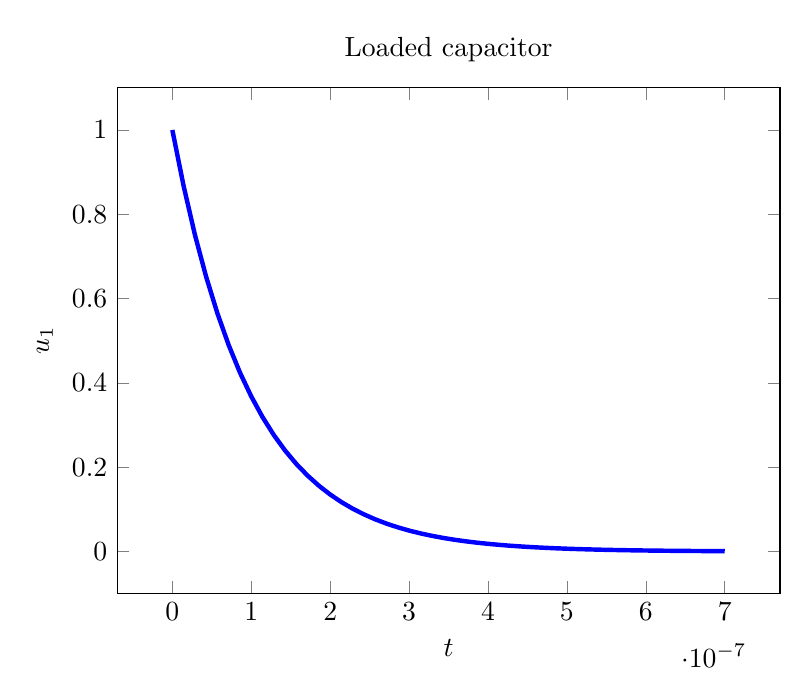
\begin{tikzpicture}
        \begin{axis}[
            samples=50,
            title=Loaded capacitor,
            xlabel={$t$},
            ylabel={$u_1$},
            width=10cm,
            height=8cm]
          \addplot[blue, ultra thick,domain=0:7e-7] ({x},{exp(-(x/(1e-7)))});
        \end{axis}
    \end{tikzpicture}
\end{frame}

\begin{frame}
\frametitle{Modified Nodal Analysis}
\begin{itemize}[<+->]
    \item Every element has a model:
        \begin{itemize}
            \item{Resistor: \(I = G \cdot U,\quad G=\frac{1}{R}\)
            \begin{description}[]
                \item[\(G\)]<.->  Conductance
            \end{description}}
            \item Capacitor: \(I = C \cdot \dot{U}\)
            \begin{description}[]
                \item[\(C\)]<.-> Capacity
            \end{description}
            \item \dots
        \end{itemize}
    \item Abstraction of the circuit as a graph \(G = (V,E)\)
    \begin{description}[]
        \item[\(V\)]<.-> Vertex
        \item[\(E\)]<.-> Edge
    \end{description}
    \item Kirchhoff's current law: \(\forall v \in V. \sum_{j \in E(v)} i_{j} = 0\)
    \begin{description}[]
        \item[\(E(v)\)] Edges connected to Vertex v
    \end{description}
\end{itemize}
\end{frame}

\begin{frame}
\frametitle{Example}
KCL: \(\forall v \in V. \sum_{j \in E(v)} i_{j} = 0\); Resistor: \(I = G \cdot U\); Cap: \(I = C \cdot \dot{U}\)
\begin{figure}[ht]
    \centering
        \begin{circuitikz}
            \draw (0,0) node[ground] {} to ++(0,1)
        -- ++(0,0) to[*R=$R$,a=$1\,\Omega$,-*] ++(2,0) node[above]{$u_1$}
        -- ++(0,0) to[*C=$C$,a=$100\,\mathrm{nF}$] ++(2,0)
        -- ++(0,0) to ++(0,-1) node[ground] {};
% \draw (3,0) to[R=1,i>_=1, o-*] (6,0);
        \end{circuitikz}
    \caption{Loaded capacitor}
\label{fig:cap}
\end{figure}
\pause
\begin{enumerate}[<+->]
    \item Concrete equation for this example:\\
        \(C\dot{u}_1 + Gu_1 = 0\)
    \item Generalization for bigger circuits:\\
        \(\mathbf{C} \dot{\vec{x}} + \mathbf{G} \vec{x} = \vec{s}(t)\)
    \item Application of generalized discretization (more later):\\
        \(\mathbf{C} (\alpha \vec{x} + \beta) + \mathbf{G} \vec{x} = \vec{s}(t)\)
    \item Prepare for Newton's method:\\
        \(\mathbf{C} (\alpha \vec{x} + \beta) + \mathbf{G} \vec{x} - \vec{s}(t)= 0\)
\end{enumerate}
\end{frame}


\subsection{Parallel Numerical Integration}
\begin{frame}
\frametitle{Problem: Inital Value Problem}
\begin{equation*}
y'(t) = f(t,y(t)), \quad y(t_0) = y_0.
\end{equation*}
\end{frame}

\begin{frame}
\frametitle{Solution*: Numerics \(\rightarrow\) discretization}
\begin{exampleblock}{Implicit Euler}
\begin{equation*}
y_{n+1} = y_n + hf(t_{n+1},y_{n+1})
\end{equation*}
\begin{equation*}
    f(t_{n+1},y_{n+1}) = \frac{y_{n+1} - y_n}{h}
    \end{equation*}
\begin{description}[]
    \item[\(h\)] stepsize
\end{description}
\pause
\begin{block}{Generalized}
    \begin{equation*}
        \dot{y}_{n+1} = \alpha \cdot y_{n+1} + \beta
    \end{equation*}
    \begin{equation*}
        \alpha = \frac{1}{h}\quad\beta = - \frac{y_n}{h}
    \end{equation*}
\end{block}
\end{exampleblock}
\pause
\begin{alertblock}{Strictly sequential}
Problematic for parallelization
\end{alertblock}
\end{frame}

